\chapter{Zastosowane oprogramowanie}

\section{Robot Operating System}

{\textbf{Robot Operating System (ROS)}} to pogramowa struktura ramowa, zawierająca zbiór bibliotek realizujących wykorzystywane w robotyce funkcje. ROS określa strukturę i mechanizmy komunikacji międzyprocesowej. Umożliwia stworzenie struktury rozproszonej, pozwalającej na wykonywanie obliczeń na wielu maszynach jednocześnie. Zasada działania opiera się na implementacji pakietów zwanych węzłami, realizujących konkretne zadania. W systemie istnieje jeden węzeł główny, poprzez którego realizowana jest komunikcja między poszczególnymi pakietami. Wymiana informacji polega na publikacji i subskrypcji wiadomości. Wiadomości nadawane są specjalnymi kanałami zwanymi tematami. Każdy węzeł może nadawać i subskrybować dowolną liczbę tematów. Same wiadomości to zbiór zmiennych, które twórca może stworzyć samodzielnie, bądź posłużyć się gotowymi wzorcami \cite{ROS}. ROS współdziała z  językami C++, Python i Lisp. \\
{\indent} ROS dostarcza abstrakcje sensorów, w tym przypadku sensorów LIDAR i Kinect, zawiera implementacje map kosztu i planerów ruchu. Istotnym pakietem jest pakiet {\textit{TF}}, który pozwala na zarządzanie wieloma systemami koordynatów \cite{prob}. \\
{\indent} W pracy wykorzystano dystrybucję ROS Kinetic z 2016r., w systemie operacyjnymUbuntu 16.04.4.

\section{Gazebo}

{\textbf{Gazebo}} jest narzędziem pozwalającym na tworzenie symulacji i ich zobrazowanie w 3D. Umożliwia implementację modeli robotów, środowiska ich pracy oraz innych elementów niezbędnych do przeprowadzenia symulacji. Modele zazwyczaj definiuje się w formacie SDF, bądź korzysta z wbudowanego kreatora. Format SDF opracowany został na bazie formatu XML, specjalnie na potrzeby opisu robotów i czujników \cite{sdf}.  Plik w formacie SDF zawiera informacje o reprezentacji graficznej modelu, modelu jego kolizji, przegubach i innych drugorzędnych parametrach. Zachowanie modelu implementowane jest poprzez specjalny mechanizm wtyczek. Podobnie definiuje się środowisko symulacji. Gazebo zawiera wbudowane cztery popularne biblioteki fizyczne: ODE, Bullet, Simbody, DART, niezależne od implementacji samej warstwy wizualnej. \\
{\indent}W bibliotece Gazebo dostępne są gotowe modele, a także opis tworzenia własnych. Odnosi się to również modeli czujników LIDAR i Kinect. Gazebo działać może niezależnie, zazwyczaj jednak wykorzystywane jest jako narzędzie zintegrowane z systemem ROS. Zaletą Gazebo jest bogate API, dzięki któremu, poprzez mechanizm wtyczek, możliwa jest implementacja zaawansowanych funkcji modeli i samej symulacji \cite{gazebo}.

\section{RVIZ}

{\textbf{RVIZ}} to narzędzie wbudowane w środowisko ROS, służące do wizualizacji aktualnego stanu systemu. Program subskrybuje zadane przez użytkownika tematy i wyświetla dane w sposób zależny od rodzaju wiadomości. Umożliwia wyświetlenie pozycji robota, map kosztu, trajektorii ruchu, chmury punktów, tzw. znaczników i innych.

\section{OpenCV}

{\textbf{OpenCV}} to biblioteka służąca do przetwarzania obrazów, zawierająca implementacje ponad stu najczęściej wykorzystywanych algorytmów. Główne funkcje biblioteki dzieli się na następujące moduły: $cv$ - funkcje główne, $imgproc$ - przetwarzane obrazu, $highgui$ - tworzenie interfejsu, object detect - detetekcja obrazów, $ml$ - uczenie maszynowe\cite{opencv}.

\section{Dlib}

{\textbf{Dlib}} jest biblioteką zawierającą implementację algorytmów uczenia maszynowego. Pozwala m.in. na tworzenie klasyfikatorów i ich wykorzystanie w celu detekcji obiektów \cite{dlib}.

\section{Symulator bazy mobilnej}

Mimo istnienia rzeczywistej bazy dookólnej, w niniejszej pracy podjęto decyzję o wykorzystaniu stworzonego wcześniej przez R. Świątkiewicza symulatora \cite{omnivelma}. Symulator ten to dokładnie odwzorowany model platformy, zaimplementowany w środowisku symulacyjnym Gazebo [\ref{fig:omnivelma_gaz}]. Zamodelowano korpus platformy, koła szwedzkie, silniki, enkodery, skandery LIDAR oraz jednostkę inercyjną i zapewniono zbliżone do pracy rzeczywistego robota działanie.

\begin{figure}[H]
	\centering
	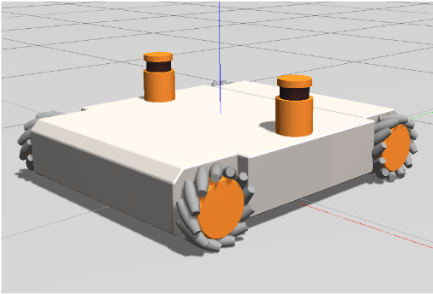
\includegraphics[width=0.5\textwidth]{gfx/omnidirectional.png}
	\caption{Model platformy w programie Gazebo \cite{omnivelma}}
	\label{fig:omnivelma_gaz}
\end{figure}

W toku prac powstał model kinematyczny i dynamiczny platformy. Poszczególne elementy zdefiniowano w plikach SDF, a następnie scalono do jednego modelu całej platformy. Zaimplementowano możliwośc odczytu z dometrii robota i umożliwiono zadawanie mu prędkości liniowej i kątowej. Możliwe jest to dzięki istnieniu modułów odpowiadających za integrację modelu z systemem ROS. Symulator publikuję wiadomości o odometrii, wynikach pomiarów sensorów LIDAR i jednostki inercyjnej korzystając z infrastruktury środowiska ROS, natomiast specjalny moduł nasłuchuje danych o zadanej prędkościach $v_{x}, v_{y}, v_{theta}$, które są przeliczane na odpowiednie prędkości poszczególnych kół platformy poprzez równanie kinematyki odwrotnej. Równanie kinematyki odwrotnej przedstawia równanie \eqref{eq:kinematic_2}. Symulator posiada również możliwość ręcznego (za pomocą klawiatury i myszy komputera) zadawnia prędkości.

\begin{figure}[H]
  	\centering 
	\begin{equation} \label{eq:kinematic_2}
	\begin{bmatrix}
	\omega_1 \\
	\omega_2 \\
	\omega_3 \\
	\omega_4 \\
	\end{bmatrix}
	=
	\frac{1}{r}
	\begin{bmatrix}
	1 & -1 & \frac{a+b}{2} \\
	1 & 1 & -\frac{a+b}{2} \\
	1 & -1 & -\frac{a+b}{2} \\
	1 & 1 & \frac{a+b}{2} \\
	\end{bmatrix}
	\begin{bmatrix}
	v_y \\
	v_x \\
	\omega_z \\
	\end{bmatrix}
	\end{equation}
	\capequation{Równanie kinematyki odwrotnej platformy \cite{omnivelma}}
\end{figure}

{\indent} Pierwotnie symulator nie przewidywał istnienia sensora Kinect, o czym mowa w implementacji. \\

{\indent} Z praktycznego punktu widzenia zastosowanie symulatora pozwala na szybszą implementację systemów mających działać z platformą. W przypadku bezpośredniego działania na robocie, należałoby przede wszystkim zapewnić jego bezpieczeństwo na każdym etapie tworzenia systemu. Sama rekompilacja kodu i ponowne uruchomienie platformy byłoby procesem znacznie bardziej czasochłonnym, gdzie w przypadku symulatora można to robić nieustannie. Zdecydowanie ułatwione jest prototypowanie, w trakcie prac można było przetestować wiele rozwiązań przed wybraniem ostatecznego. W przypadku tworzenia i testów podsystemów detekcji człowieka, ktoś nieustannie musiałby fizycznie znajdować sie przy robocie, co jest praktycznie niemożliwe. \\ 
{\indent}Z założenia natomiast system powstały na bazie symulacji nie różni się wiele od tego, który ostatecznie będzie mógł zostać uruchomiony na robocie. 